\providecommand{\main}{..}

\documentclass[../principal]{subfiles}

\begin{document}
\espacio

  En este capítulo se realiza una comparación de costos entre el sistema propuesto y uno de características similares que se puede encontrar en el mercado. Se realiza un análisis de vulnerabilidades observadas en el sistema desarrollado y los pasos a seguir para evitar ataques o fallas en el sistema. Por último se muestran los resultados de la instalación piloto ejecutada en la Agencia para el Desarrollo de la Sociedad de la Información en Bolivia.

  \section{Análisis de costos}

  Para poder justificar la reducción de costos, se realizó el análisis de costos de un sistema similar. Este análisis se estructuró en tres etapas: la instalación del controlador central, la instalación de los sensores en cada puerta y la instalación de las cerraduras de cada puerta.

  Existe un sistema similar fabricado por la industria \href{http://www.zksoftware.com.ar/control_accesos.php}{ZKSoftware}, este tiene un controlador central que puede abastecer como máximo un número de 4 puertas, pero se le puede añadir módulos para incrementar el control de más puertas, módulos de Sensor de huellas, RFID o rostros. La ventaja de este sistema es que almacena hasta 3000 huellas, el sistema desarrollado solo puede almacenar hasta 1000 huellas, la desventaja es que solo tiene compatibilidad con los sensores, cerraduras, etc, de la misma marca. Cuenta con un servidor web que permite administrar fácilmente los permisos de acceso al igual que el sistema desarrollado. Otra desventaja de este sistema ZKSoftware es que todos los módulos de expansión de control de puertas deben estar conectados al controlador central, pero el sistema desarrollado solo necesita una conexión de red que comunique al servidor MQTT con los controladores sin importar la infraestructura que exista en medio.

  \subsection{Costo del dispositivo de control central}

  La tabla \ref{tabla:costo_controlador} muestra la comparación entre el sistema con más características similares que se puede encontrar en el mercado y el sistema propuesto en este proyecto.

  \begin{center}
    \begin{longtable}{|>{\centering\arraybackslash}p{4cm}|>{\centering\arraybackslash}p{5cm}|>{\centering\arraybackslash}p{5cm}|}
      \caption{Comparación de costos para el dispositivo de control}
      \\
        \hline
        \rowcolor[HTML]{FFEAD0}
        Característica & Placa de control ZKSoftware & Placa de control desarrollada \\
        \hline
      \endfirsthead
      \multicolumn{3}{c}{\tablename\ \thetable\ -- Comparación de costos para el dispositivo de control (continuación)}
      \\
        \hline
        \rowcolor[HTML]{FFEAD0}
        Característica & Placa de control ZKSoftware & Placa de control desarrollada \\
        \hline
      \endhead
      \multicolumn{3}{c}{\textit{Continua en la página siguiente}} \\
      \endfoot
      \endlastfoot
        Modelo & InBIO-460 & Placa de control POE \\
        \hline
        Cantidad de puertas & 6 & 6 \\
        \hline
        Cantidad de sensores & 6 & \makecell[{{p{5cm}}}]{Puertos del switch POE \\ Máximo 10000} \\
        \hline
        Accesorios necesarios & Expansión InBIO 260 & \makecell[{{p{5cm}}}]{Módulo de relés \\ Switch POE} \\
        \hline
        Capacidad de huellas & 3000 & 1000 \\
        \hline
        CPU & 32bit @ 400Mhz & 8bit @ 16Mhz \\
        \hline
        Memoria RAM & 32MB & 2KB \\
        \hline
        Memoria Flash & 128MB & 32KB \\
        \hline
        Conexión con los sensores & RS485 & TCP/IP \\
        \hline
        Puertos de entrada & \makecell[{{p{5cm}}}]{4 Botón de salida \\ 4 Sensor de puerta abierta \\ 4 auxiliares \\ +2 Botón de salida \\ +2 Sensor de puerta abierta \\ +2 auxiliares} & 6 Pines de control de cerraduras \\
        \hline
        Pines de salida & \makecell[{{p{5cm}}}]{4 Relés para cerraduras \\ 4 Auxiliar \\ +2 Relés para cerraduras \\ +2 Auxiliar} & 6 Relés para cerraduras \\
        \hline
        Indicador LED & LED de estado & \makecell[{{p{5cm}}}]{LED de estado de energía \\ LED de conexión con el servidor \\ LED de conexión de red \\ LED de transmisión de datos} \\
        \hline
        Fuente de alimentación & DC 9.6V-14.4V & POE 802.3af - 48V \\
        \hline
        Dimensiones & 218mm x 106mm x 36mm & 94mm x 64mm x 17mm \\
        \hline
        Software & ZKAccess (Con licencia) & Código abierto \\
        \hline
        Costo del equipo & 527\$us & 40\$us \\
        \hline
        Costo de accesorios & 313\$us & 272\$us \\
        \hline
        \textbf{Costo total} & \textbf{840\$us} & \textbf{312\$us} \\
        \hline
      \caption*{\textbf{Fuente:} Elaboración propia}
      \label{tabla:costo_controlador}
    \end{longtable}
  \end{center}

  Los datos de los precios fueron adquiridos de las tiendas virtuales \href{http://articulo.mercadolibre.com.co/MCO-442917237-controladora-biometrica-inbio-460-_JM}{mercadolibre.com.co} y \href{http://tecbolivia.com/index.php/venta-de-componentes-electronicos-11/actuadores/modulo-relay-de-4-canales-5v-detail}{www.tecbolivia.com}.

  \subsection{Costo del dispositivo de interfaz sensorial}

  Se analizó el costo de instalación de un sensor en una sola puerta; para la comparación se tomó en cuenta un dispositivo que se pueda encontrar en el mercado y que sea compatible con el controlador mostrado en la tabla \ref{tabla:costo_controlador}.

  \begin{center}
    \begin{longtable}{|>{\centering\arraybackslash}p{4cm}|>{\centering\arraybackslash}p{5cm}|>{\centering\arraybackslash}p{5cm}|}
      \caption{Comparación de costos para el dispositivo interfaz sensorial}
      \\
        \hline
        \rowcolor[HTML]{FFEAD0}
        Característica & Lector de huella ZKSoftware & Placa de interfaz desarrollada \\
        \hline
      \endfirsthead
      \multicolumn{3}{c}{\tablename\ \thetable\ -- Comparación de costos para el dispositivo interfaz sensorial (continuación)}
      \\
        \hline
        \rowcolor[HTML]{FFEAD0}
        Característica & Lector de huella ZKSoftware & Placa de interfaz desarrollada \\
        \hline
      \endhead
      \multicolumn{3}{c}{\textit{Continua en la página siguiente}} \\
      \endfoot
      \endlastfoot
        Modelo & FR-1500WP & Placa interfaz POE \\
        \hline
        Accesorios necesarios & \makecell[{{p{5cm}}}]{Convertidor RS485 a RJ45 \\ Cable ethernet cat. 5E de 100ft de longitud} & \makecell[{{p{5cm}}}]{Sensor de huellas \\ Cable ethernet cat. 5E de 100ft de longitud} \\
        \hline
        Protección & IP65 & Ninguna \\
        \hline
        Tipo de sensor & Óptico & Óptico \\
        \hline
        Fuente de alimentación & DC 12V & POE 802.3af - 48V \\
        \hline
        Dimensiones & 121.3mm x 77.3mm x 38mm & 94mm x 64mm x 17mm \\
        \hline
        Consumo en análisis de huella & 140mA & 100mA \\
        \hline
        CPU & 1GHz & 16MHz \\
        \hline
        Sensor & SilkID & ZFM-20 \\
        \hline
        LED & Indicador de tres colores & Indicador de lectura de huella \\
        \hline
        Compatibilidad & \makecell[{{p{5cm}}}]{Paneles InBIO \\ Paneles InBIO Pro} & Código abierto \\
        \hline
        Costo del equipo & 310\$us & 40\$us \\
        \hline
        Costo de accesorios & 56\$us & 66\$us \\
        \hline
        \textbf{Costo total} & \textbf{366\$us} & \textbf{106\$us} \\
        \hline
      \caption*{\textbf{Fuente:} Elaboración propia}
      \label{tabla:costo_sensor}
    \end{longtable}
  \end{center}

  \subsection{Costo de la cerradura de cada puerta}

  Este paso de la instalación fue analizado tomando en cuenta una sola cerradura, la comparación se realizó entre una cerradura compatible con el sistema hallado en el mercado y una compatible con el sistema propuesto en este proyecto.

  \begin{center}
    \begin{longtable}{|>{\centering\arraybackslash}p{4cm}|>{\centering\arraybackslash}p{5cm}|>{\centering\arraybackslash}p{5cm}|}
      \caption{Comparación de costos para la cerradura magnética}
      \\
        \hline
        \rowcolor[HTML]{FFEAD0}
        Característica & Cerradura magnética ZKSoftware & Cerradura magnética Syscom \\
        \hline
      \endfirsthead
      \multicolumn{3}{c}{\tablename\ \thetable\ -- Comparación de costos para la cerradura magnética (continuación)}
      \\
        \hline
        \rowcolor[HTML]{FFEAD0}
        Característica & Cerradura magnética ZKSoftware & Cerradura magnética Syscom \\
        \hline
      \endhead
      \multicolumn{3}{c}{\textit{Continua en la página siguiente}} \\
      \endfoot
      \endlastfoot
        Modelo & YB700B & YB300 \\
        \hline
        Accesorios necesarios & \makecell[{{p{5cm}}}]{Botón pulsador ABK800A \\ Cable ethernet categoría 5-E de 100ft de longitud} & \makecell[{{p{5cm}}}]{Botón pulsador Saxxon RB03 \\ Cable ethernet categoría 5-E de 100ft de longitud} \\
        \hline
        Tiempo de retardo & 0/3/6/9s & 0/3/6/9s \\
        \hline
        Fuente de alimentación & 12-24V & 12-24V \\
        \hline
        Consumo de corriente & \makecell[{{p{5cm}}}]{12V/900mA 12V/120mA \\ 24V/730mA 24V/80mA } & \makecell[{{p{5cm}}}]{12V/900mA 12V/130mA \\ 24V/730mA 24V/90mA } \\
        \hline
        Dimensiones & 205mm x 35mm x 41mm & 205mm x 35mm x 41mm \\
        \hline
        Diámetro pestillo & 16mm & 16mm \\
        \hline
        Peso & 0.7Kg & 0.7Kg \\
        \hline
        Fuerza de sujeción & 1000Kg & 1000Kg \\
        \hline
        Señal de salida & NC/COM & NC/COM \\
        \hline
        N\degree{} operaciones & 500000 & 500000 \\
        \hline
        Costo del equipo & 87\$us & 54\$us \\
        \hline
        Costo de accesorios & 25\$us & 23\$us \\
        \hline
        \textbf{Costo total} & \textbf{112\$us} & \textbf{77\$us} \\
        \hline
      \caption*{\textbf{Fuente:} Elaboración propia}
      \label{tabla:costo_cerradura}
    \end{longtable}
  \end{center}

  \section{Análisis de vulnerabilidades}\label{sec:analisis_vulnerabilidades}

  El sistema desarrollado cumple con los siguientes estándares de la Norma Boliviana NB-1220004\cite{norma:nb_1220004}:

  \begin{itemize}
    \item Señales táctiles en los pulsadores de salida al interior de cada puerta, secciones 2.1.2.2(pp. 30) y 5.4(pp. 161)
    \item Ubicación de señales visuales, sección 2.2 (pp. 31)
    \item Características de las puertas corredizas y de vaivén, sección 3.4 (pp. 148)
  \end{itemize}

  La caja metálica donde se halla el control central del sistema cumple con los siguientes estándares de la Norma Boliviana RM-849-14\cite{norma:rm_849_14}:

  \begin{itemize}
    \item Cuenta con señales de advertencia de peligro por electrocución, sección 2.1.4(pp. 16)
    \item El camino a las puertas está marcado con señales de evacuación, sección 2.1.5(pp. 20-21)
  \end{itemize}

  El sistema también cumple los estándares de la norma internacional NFPA-730\cite{norma:nfpa_730}:

  \begin{itemize}
    \item Los ambientes cumplen con la definición de ``Área Controlada'', secciones 3.3.5.1(pp. 9) y 8.2.1 (pp. 41)
    \item Las cerraduras son de tipo electrónicas, secciones 7.2.1 (pp. 29) y 7.2.3(pp. 30-31)
    \item Las puertas corredizas tienen protección antibandálica y no se pueden remover fácilmente para extraerlas de sus rieles, secciones 7.3.6.5 (pp. 34) y 7.3.6.6 (pp. 34)
    \item El sistema desarrollado cumple con la definición de ``Sistema de Control de Acceso'' de tipo Portal-Múltiple, secciones 8.13.1 (pp. 44-45) y 8.13.1.2 (pp. 45)
    \item La identificación se realiza mediante Verificación de Huellas Dactilares y se habilitan mediante sensores biométricos con la posibilidad de definir permisos con fechas definidas de inicio y fin, secciones 8.13.3 (pp. 47) y 8.13.3.1 (pp. 47)
    \item Cuenta con la posibilidad de instalar una o más Estaciones Monitoras, sección A3.3.35 (pp. 106)
  \end{itemize}


  El sistema es respaldado mediante un sistema de video-vigilancia que captura en video de manera ininterrumpida todos los ingresos y salidas de personas del centro de datos. La energía es suministrada al sistema mediante una UPS de respaldo en caso de fallas en la red eléctrica durante el tiempo necesario en el cual se activa un generador a diésel como se especifica en la Norma Internacional NFPA-731 en el capítulo 6 (pp. 21-23), pero se dejó de lado la encriptación de datos que requiere un hardware especializado cuya definición se encuentra en la sección 6.3 (pp. 23) de la misma norma. \cite{norma:nfpa_731}

  Por de ello este sistema no garantiza el nivel de seguridad en la capa SSL a través de TLS del estándar ISO/IEC PRF 20922\footnote{\href{https://www.iso.org/standard/69466.html}{Message Queuing Telemetry Transport v3.1.1}} ya que los dispositivos desarrollados tan solo conllevan la seguridad de conexión mediante credenciales de usuario/contraseña, por lo cual el sistema es vulnerable ante ataques de interceptación con algún software como WireShark mediante el cual se puede monitorear la red para observar cada paquete que se intercambia de un host a otro utilizando una tarjeta de red conectada físicamente a la misma red en modo promiscuo. Con este método se pueden ver en claro los usuarios y contraseñas de los dispositivos al momento de la conexión al servidor MQTT ya que éste levanta el servicio en el puerto 1883 y no en el puerto 8883. Para evitar este problema es recomendable aislar físicamente la red donde se encuentran conectados los dispositivos y de esta manera evitar la intrusión de atacantes.

  Otra de las vulnerabilidades que se puede hallar en este y en cualquier sistema electrónico de seguridad se produce con una falla en la energía, este sistema no puede estar desprovisto de energía ya que las cerraduras magnéticas se liberan y las puertas se abren, quedando desprotegida el área donde se instaló el sistema. Para evitar este problema se recomienda aislar la energía eléctrica de este sistema, conectando todos los dispositivos a un respaldo de energía UPS; si las áreas que se van a resguardar son de alta criticidad además se tendrá que instalar un generador eléctrico alternativo o bien alimentar a la UPS con un banco de baterías.

  Las bases de datos desarrolladas para este sistema tienen un grado de protección contra inyección SQL, pero aún así se recomienda configurar el servidor para que solo algunas direcciones IP tengan acceso a las dos bases de datos y cambiar el puerto de escucha por defecto al momento de la instalación.

  Los sensores de huellas dactilares ZFM-20 vienen por defecto con una dirección hexadecimal de 4bytes $ ffffffffH $, el manual de instalación del sistema tiene la posibilidad de cambiar esta dirección. Se recomienda cambiar la dirección de cada sensor antes de instalarlo en el sistema ya que una persona con el conocimiento del flujo y los protocolos de comunicación podría retirar un sensor y conectar un dispositivo que emule el funcionamiento del mismo, con lo cual podría realizar ataques de fuerza bruta para abrir alguna puerta del sistema. Para evitar este tipo de ataque se recomienda también instalar un respaldo en cuanto a la seguridad en los ambientes como cámaras que apunten o enfoquen a los lugares donde se hallan los sensores para tener una respuesta temprana en caso de actividad sospechosa. Cabe mencionar que el sistema desarrollado es compatible con otros sistemas de seguridad, ya que los esquemáticos son también hardware libre y están disponibles para realizar adaptaciones; por ejemplo con un sistema de detección de gases o elementos nocivos en el aire, se puede lograr abrir las puertas en caso de emergencia con sólo un programa que publique el mensaje de apertura de cada puerta en los tópicos correspondientes del servidor MQTT.

  En cuanto a los permisos de acceso temporal, éstos se brindan únicamente definiendo dos fechas, una inicial y la otra final, no se toma en cuenta una hora en ninguno de los dos datos, por lo cual las personas con permiso de acceso temporal podrán ingresar a los ambientes desde las 00:00 horas de la fecha inicial hasta las 24:00 horas de la fecha final. Aún así, dada la naturaleza del software libre, éste algoritmo es pasible a cambios y adaptaciones para cada caso particular donde se necesite otro tipo de discriminación para los accesos temporales.

  Para el sistema web se seleccionó el método de sesiones mediante tokens en formato JSON ya que este formato es compatible con dispositivos móviles como tablets o smartphones, pero se incluyó la encriptación de los tokens en el lado del servidor y se eliminó la información crítica como las contraseñas o los ID de usuario evitando de esta manera el ataque mediante la desencriptación por fuerza bruta de los tokens. Pero el problema que se genera en cualquier sistema web se debe también a motivos de descuido humano, ya que no se puede controlar el hecho de que algunas personas dejen sus cuentas abiertas o anoten sus credenciales de forma física en hojas de papel, entonces mediante este tipo de descuidos un atacante podría acceder al sistema con las credenciales de otra persona y abrir las puertas por las cuales tiene acceso la persona que descuidó sus credenciales. Las personas con acceso al sistema deberán capacitarse de manera periódica a fin de evitar este tipo de descuidos.

  \section{Resultados de la prueba piloto}

  Por razones de seguridad no se proporcionan detalles a profundidad de los ambientes o los datos utilizados en la prueba piloto, pero se pueden mencionar los aspectos generales de los resultados de dicha prueba para demostrar la reducción del costo en caso de instalar un sistema similar que se puede encontrar en el mercado.

  El sistema fue implantado en todos los ambientes del centro de datos de la Agencia para el Desarrollo de la Sociedad de la Información en Bolivia, cada puerta cuenta con un dispositivo interfaz sensorial, un sensor de huellas ZFM-20, una cerradura magnética, un botón pulsador en el interior de cada ambiente, donde todas las conexiones se realizaron con cable UTP Categoría 5-E.

  Cada dispositivo es alimentado mediante POE a través de un switch al cual también se conecta un dispositivo de control central que abastece para el número de puertas necesarias del sistema. Cada uno de los dispositivos fue grabado con el programa que genera el mismo sistema, por lo cual cada dispositivo tiene un usuario definido y una contraseña aleatoria. Cuando el administrador decide actualizar el sistema o cambiar uno de los dispositivos las contraseñas vuelven a generarse siempre de manera aleatoria de forma automática.

  El método para grabar los programas en los dispositivos es mediante la conexión ISP disponible en la placa del circuito desarrollado. El administrador del sistema debe registrar un nuevo dispositivo para que el sistema habilite la opción de generar el programa a ser grabado. Para este proceso es necesario un dispositivo adaptador USB-ISP como el que se muestra en la figura \ref{fig:programador_usb_isp}.
  
  \begin{figure}[H]
    \centering
    \caption{Programador USB-ISP}
    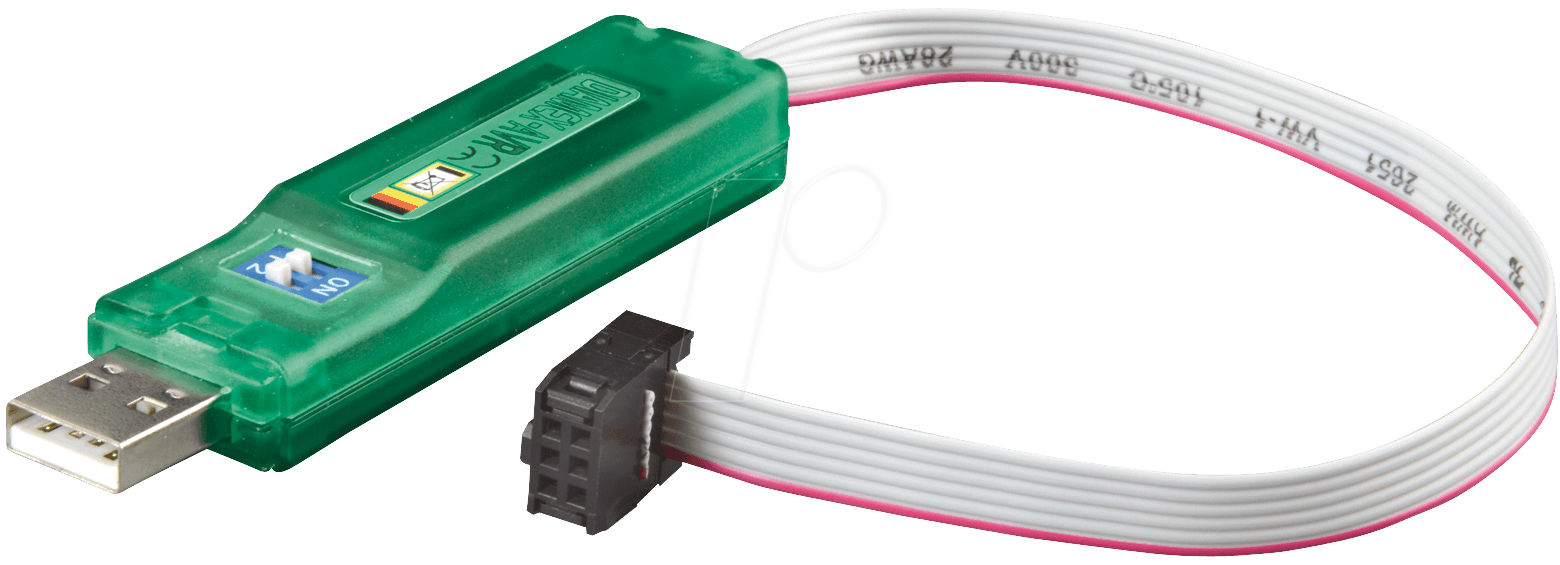
\includegraphics[width=0.7\textwidth]{analisis/programador_usb_isp.png}
    \caption*{\textbf{Fuente:} \href{https://www.reichelt.de/Programmer-Entwicklungstools/DIAMEX-USB-ISP/3/index.html?ACTION=3&GROUPID=2969&ARTICLE=110344&OFFSET=16&SID=12VLdmv38AAAIAABPfxBE17abb04ab6a2ccacf919af2833668124&LANGUAGE=EN}{Tienda virtual Reichelt Electronik, Alemania, 2017}}
    \label{fig:programador_usb_isp}
  \end{figure}

  Las dos bases de datos, el servidor MQTT y la API de administración se hallan en un servidor aislado de la red al cual se accede solo desde equipos con una dirección MAC e IP específicas mediante reglas de un enrutador que comunica dos redes.

  En la misma red del cliente que tiene acceso al servicio web de administración se conecta el dispositivo registrador de huellas para que éste pueda subir los datos de las huellas registradas a la base de datos sólo cuando el administrador conecta el equipo y prepara la grabación de una nueva huella.

  Los materiales utilizados y el costo de instalación del sistema se muestran en la tabla \ref{tabla:costo_prueba_piloto}. En esta tabla no se contemplan los trabajos de remodelación necesarios en la infraestructura como el de picar las paredes para insertar los ductos, los materiales de construcción para arreglar los desperfectos necesarios para la instalación como estuco o cemento, ni tampoco los materiales necesarios para recubrir y enmascarar la instalación como la pintura o el cemento adhesivo.

  \begin{landscape}
    \begin{center}
      \begin{longtable}{|>{\centering\arraybackslash}p{2.5cm}|>{\centering\arraybackslash}p{2.5cm}|>{\centering\arraybackslash}p{3cm}|>{\centering\arraybackslash}p{5cm}|>{\centering\arraybackslash}p{2.5cm}|>{\centering\arraybackslash}p{2.5cm}|}
        \caption{Materiales y presupuesto utilizados en la instalación piloto}
        \\
          \hline
          \rowcolor[HTML]{FFEAD0}
          Tipo & Categoría & Recurso & Descripción & Cantidad & Monto \$us\\
          \hline
        \endfirsthead
        \multicolumn{6}{c}{\tablename\ \thetable\ -- Materiales y presupuesto utilizados en la instalación piloto (continuación)}
        \\
          \hline
          \rowcolor[HTML]{FFEAD0}
          Tipo & Categoría & Recurso & Descripción & Cantidad & Monto \$us\\
          \hline
        \endhead
        \multicolumn{6}{c}{\textit{Continua en la página siguiente}} \\
        \endfoot
        \endlastfoot
          \multirow{3}{\linewidth}{Recursos disponibles} & \multirow{3}{\linewidth}{Infraestructura} & Equipo & Servidor broker MQTT & 1 equipo & \\
          & & Equipo & Servidor de base de datos & 1 equipo & \\
          & & Material & Alicates, desarmadores, estación de soldar, taladro, cierra mecánica, etc & 1 pieza & \\
          \hline
                \multirow{9}{\linewidth}{Recursos necesarios} & \multirow{9}{\linewidth}{Materiales} & Electrónico & Ethernet Cat. 5-E & 3 cajas & 423 \\
          & & Material & Switch POE de 24 puertos & 1 equipo & 280 \\
          & & Eléctrico & Cable 4 hilos para teléfono & 2 cajas & 58 \\
          & & Eléctrico & Disyuntor & 1 pieza & 10 \\
          & & Eléctrico & Borneras y fusibles & 15 piezas & 20 \\
          & & Eléctrico & Chapas magnéticas 12V & 5 piezas & 270 \\
          & & Eléctrico & Fuentes de 12V & 5 piezas & 100 \\
          & & Eléctrico & Fuente de 5V & 1 piezas & 20 \\
          & & Electrónico & Dispositivo interfaz sensorial & 5 piezas & 530 \\
          & & Electrónico & Dispositivo control central & 1 piezas & 104 \\
          & & Electrónico & Pulsador interno de pared & 5 piezas & 35 \\
          & & Electrónico & Patch panel de 24 puertos & 1 pieza & 26 \\
          & & Material & Tubos conduit, cable-ductos, tubos PVC & 90 metros & 100 \\
          & & Material & Gabinete empotrable IP65 con cerradura & 1 pieza & 86 \\
          & & Material & Termocontraibles, conectores, cables jumper hembra-hembra, cables jumper hembra-macho, cables jumper macho-macho, conectores RJ45 & 4 metros & 65 \\
          & & Material & Tornillos y tuercas & 100 piezas & 20 \\
          \hline
          \multicolumn{5}{|c|}{\bf{Costo total (\$us)}} & \bf{2147} \\
          \hline
        \caption*{\textbf{Fuente:} Elaboración propia}
        \label{tabla:costo_prueba_piloto}
      \end{longtable}
    \end{center}
  \end{landscape}

  Realizando una comparación de costos con las tablas \ref{tabla:costo_controlador}, \ref{tabla:costo_sensor} y \ref{tabla:costo_cerradura} se obtiene el resultado de que un sistema de la misma escala llegaría a tener un precio de aproximadamente 3230\$us, a diferencia del sistema propuesto que tuvo un costo de 2147\$us, con lo que se obtuvo una reducción del 33.5\% del costo en la instalación del sistema en los cinco ambientes para la prueba piloto.

  Pero no debemos olvidar que no se tomaron en cuenta los recursos que la entidad ya tenía disponibles como por ejemplo los servidores o las herramientas para la instalación.

  Este proceso fue realizado con la aprobación del Director Ejecutivo de ADSIB, Sylvain Damien Lesage, quien verificó el correcto funcionamiento del sistema al finalizar la instalación, realizó las pruebas correspondientes y calificó la instalación como favorable para la seguridad del centro de datos de dicha entidad.

  La aprobación del Director Ejecutivo de ADSIB se remitió por escrito a mi persona como se puede observar en el Anexo \ref{anx:instalacion_piloto_documento}.

  \bibliografia

\end{document}
